%!TEX program = xelatex

% 纸张模式:护眼模式-geye 朦胧模式-hazy
% 纸张尺寸:pad kindle pc normal screen
\documentclass[cn, blue, normal, 12pt]{elegantnote}

\title{软件工程复习笔记}
\author{Xiaohei}
\institute{\href{https://github.com/Moby-C/SoftwareEngineeringNote}{GitHub Page}}
\version{1.1}
\date{\zhtoday}

\begin{document}

\maketitle

\section{软件工程学概述}

复习内容:

\begin{enumerate}
    \item 了解软件工程的诞生及软件的特点
    \item 了解软件危机
    \item 掌握软件工程的三个基本要素
    \item 了解软件生命周期的含义及各阶段的任务
    \item 了解软件过程各模型的适用范围
\end{enumerate}

\subsection{软件工程学}

迄今为止,人们仍然没有彻底摆脱“\textbf{软件危机}”的困扰,软件已经成为限制计算机系统发展的瓶颈。软件工程概念的提出是为了解决\textbf{软件危机}。

软件工程的诞生:1968年北大西洋公约组织召开国际会议,提出“软件工程”概念和术语。

软件工程的目标:创造“\textbf{足够好}”的软件。

\subsection{软件的特点}

软件包括:为实现设计的功能和性能要求的\textbf{指令集};使程序能正常运行的\textbf{数据};与程序开发、维护和使用有关的\textbf{文档}。

\subsection{软件危机}

软件危机就是指在软件开发和软件维护过程中所存在的一系列\textbf{严重问题}。

产生软件危机的原因:软件具有\textbf{复杂性}、\textbf{演化性}、\textbf{服从性}、\textbf{不可见性}。

\subsection{软件生命周期}

软件生命周期指一个软件\textbf{从提出开发要求开始直到不再使用(报废)为止}的整个时期。

软件生存周期阶段划分为三个时期:\textbf{软件定义、软件开发、软件使用和维护}。

软件定义时期:问题定义、可行性研究、需求分析。

软件开发时期:概要设计、详细设计、编码及单元测试、综合测试。

软件维护时期:改正性维护、适应性维护、完善性维护、预防性维护。

\subsection{软件工程方法学}

软件工程方法学的三要素:\textbf{过程、方法、工具}。

\subsection{软件过程}

\textbf{软件过程}描述为了开发出客户需要的软件,什么人、在什么时候、做什么事以及怎样做这些事以实现某一个特定的具体目标。

\textbf{软件过程模型}定义软件开发过程中所需要完成的活动、活动之间的顺序以及活动之间的关系。

\subsubsection{瀑布模型}

瀑布模型也称经典生命周期模型,开发阶段严格按照线性方式进行
,每一个阶段具有相关的里程碑和交付产品,且需要确认和验证。

瀑布模型适用于\textbf{系统需求明确且稳定、技术成熟、工程管理较严格}的场合。如军工、航天、医疗。

\subsubsection{快速原型模型}

快速原型是快速构建一个可运行的软件原型,用户和开发人员通过对原型的检查来决定原型是否合适和恰当。

快速原型模型适用于\textbf{客户不清楚系统的具体输入输出,开发者不确定算法效率、计算机交互的方式}等场合。

\subsubsection{增量模型}

把软件产品作为一系列的增量构件来设计、编码、集成和测试。每
个构件由多个相互作用的模块构成,并且能够完成特定的功能。

增量模型适用于\textbf{软件开发中需求可能发生变化、具有较大风险、或者希望尽早进入市场}的项目。

\subsubsection{Rational统一过程模型}

由Rational公司推出的完整的软件工程方法,已获得广泛使用。基于面向对象方法学,使用统一建模语言UML(Unified Modeling Language),适合\textbf{大团队、大项目}。

\subsubsection{敏捷开发过程}

敏捷开发是一种基于更紧密的团队协作、能够有效应对快速变化需求、快速交付高质量软件的迭代和增量的新型软件开发方法。

敏捷开发过程适用于\textbf{需求模糊且经常改变的场合},适合\textbf{商业竞争环境下的项目}。

最有影响的两个敏捷开发方法是Scrum开发方法和极限编程(XP)。

\section{需求分析}

复习内容:

\begin{enumerate}
    \item 了解面向过程和面向对象分析模型有哪些描述工具
    \item 掌握数据流图
    \item 掌握数据字典的定义、作用和组成条目
    \item 掌握用例图
    \item 了解类图的组成和类与类之间的关系
    \item 了解其他需求分析阶段的图形工具
    \item 掌握验证软件需求的正确性的四个方面
\end{enumerate}

\subsection{分析模型的描述工具}

\begin{table}[htbp]
    \centering
    \begin{tabular}{c|c|c}
    \toprule
            & 面向过程的需求分析 & 面向对象的需求分析   \\
    \midrule
    数据模型 & 实体-联系图、数据字典 & 类图、类关系图   \\
    功能模型 & 数据流图(DFD)    & 用例图             \\
    行为模型 & 状态变迁图(STD) & 活动图、时序图、状态图 \\
    \bottomrule
    \end{tabular}
\end{table}

\subsection{数据流图}

数据流图是从数据传递和加工的角度,以图形的方式刻画数据流从输入到输出的移动变换过程。

\textbf{数据流}是数据在系统中的传送通道,数据流符号的箭头指明了数据的流动方向,由一组固定成分的数据组成。数据流可从加工流向加工,也可在加工与数据存储或外部项之间流动;两个加工之间可有多股数据流。

\textbf{加工}表示对数据进行的操作,如“处理选课单” 等。每个加工至少有一个输入数据流和一个输出数据流。加工的编号是这个加工在层次分解中的位置。

\textbf{数据存储}是用于保存数据的数据文件,它可以是数据库文件或
任何其他形式的数据组织。

\textbf{外部实体}(数据源点/终点)是反映数据流图与外部实体之间的联系,表示图中的输入数据来自哪里或处理结果送向何处。

\begin{figure}[htbp]
    \centering
    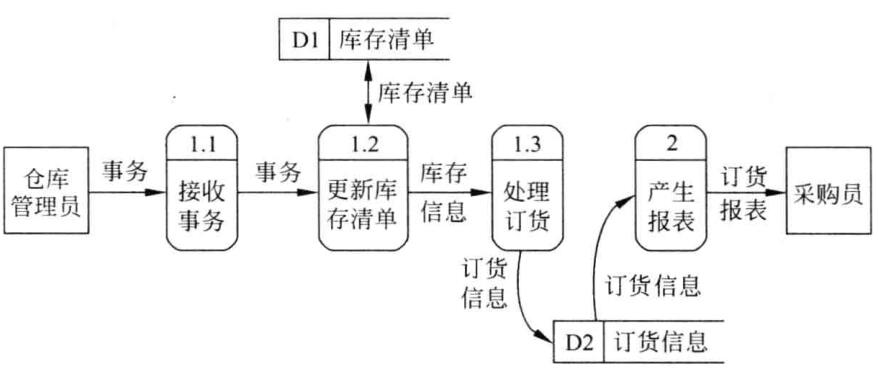
\includegraphics[width=0.8\textwidth]{数据流图.jpg}
\end{figure}

\subsection{数据字典}

\textbf{数据字典}是数据流图的补充,能够准确地定义数据流图中各组成成分的具体含义。

数据字典用简洁、清晰、易理解的文字描述条目,说明数据流图的加工功能、性能、要求及设计约束等。

数据流图和数据字典共同构成了系统的功能逻辑模型。

数据字典的组成:\textbf{数据流条目、数据项条目、数据文件条目、数据加工条目}。

\subsection{用例图}

用例建模用于描述系统需求,把系统当作黑盒,从用户的角度,描述系统的场景。主要的图形元素有:参与者、用例。

\textbf{参与者}:是指外部用户或外部实体在系统中扮演的角色。 可以是一个人、一个硬件设备等。

\textbf{用例}:对一组动作序列的描述,系统通过执行这一组动作序列为参与者产生一个可观察的结果。用例名往往用动宾结构命名。

\textbf{系统}:用于界定系统功能范围,描述该系统功能的用例都置于其中,而描述外部实体的参与者都置于其外。

用例图中的四种关系:\textbf{关联、泛化、包含、扩展}。

\textbf{关联}:参与者与用例之间的通信,任何一方都可发送或接受消息。箭头指向消息接收方。

\textbf{泛化}:就是通常理解的继承关系,子用例和父用例相似,但表现出更
特别的行为;子用例可以重载父用例。父用例通常是抽象的。箭头由子用例指向父用例,箭头为空箭头。

\textbf{包含}:当多个用例有共享行为时,应该使用包含的关系来表示它们。箭头由基本用例指向共享用例,连线为虚线。

\textbf{扩展}:扩展关系是指用例功能的延伸,相当于为基础用例提供一个附加功能。 由一个用例的扩展点可以扩展出另外一个用例。箭头指向基础用例,连线为虚线。

包含关系中,在执行基本用例时,一定会执行包含用例部分;扩展关系中,一个基本用例执行时,可以执行或不执行扩展用例部分。

\begin{figure}[htbp]
    \centering
    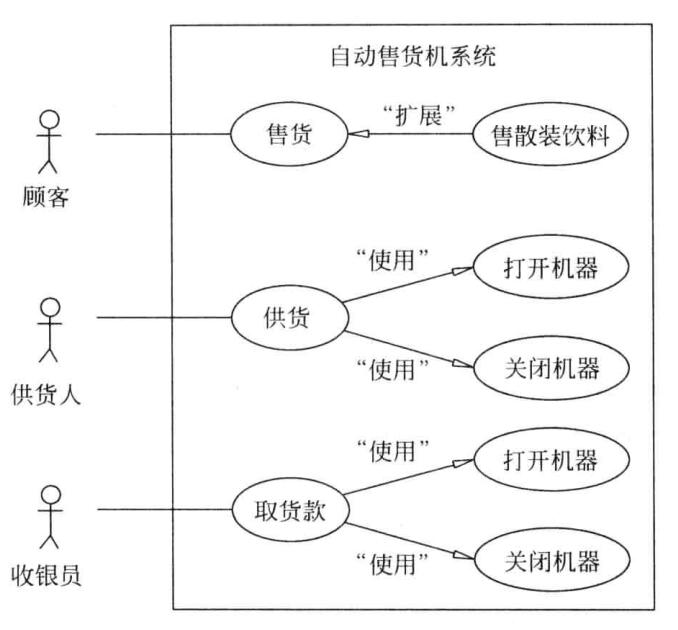
\includegraphics[width=0.5\textwidth]{用例图.jpg}
\end{figure}

\subsection{类图}

类图是由若干类关联在一起,反映系统或者子系统组成结构的静态图。

类图的组成:\textbf{类、关联}。

\textbf{类}:是具有共同结构特征、行为特征、联系和语义的对象集合的抽象形式。

\textbf{关联}:表示类与类之间的关系。

类在UML中通常以实线矩形框表示,矩形框中含有若干分隔框,分别包含类的名字、属性、操作、约束以及其他成分等。

类的属性在UML类图标的矩形框中用文字串说明。“:”后跟属性值的数据类型,可通过在属性名和数据类型后添加“=”为属性指定初始值。

操作(方法)是类提供的功能服务,在类矩形框中用文字串说明。

类的关系:\textbf{关联关系(聚合、组合)、依赖关系、泛化关系}等。

\textbf{关联关系}:\textbf{聚合}描述整体和部分的关系,其中一个类为整体,它由一个或多个部分类组成。在聚合中,部分类可以没有整体类而存在。聚合使用\textbf{带有空心菱形的实线}连接。\textbf{组合}是特殊的聚合关联。组合关联中组成整体类的部分类不能独立存在,需要整体类才能存在。组合使用\textbf{带有实心菱形的实线}连接。

\textbf{依赖关系}:指一个类的元素使用了另一个类。依赖关系描述类之间的引用关系。使用\textbf{带箭头的虚线}连接。

\textbf{泛化关系}:描述类之间的继承关系。利用泛化来表达类之间的相似性,子类共享父类的属性和操作。使用\textbf{带空心箭头的实线}连接。

\begin{figure}[htbp]
    \centering
    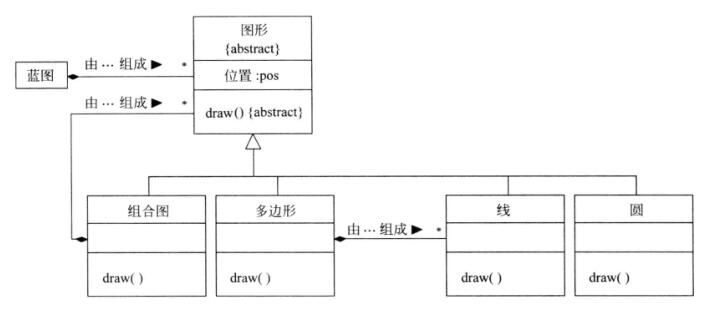
\includegraphics[width=1.0\textwidth]{类图.jpg}
\end{figure}

\subsection{其他图形工具}

\textbf{状态转换图}:通过描绘系统的状态及引起系统状态转换的事件,来表示系统的行为。状态图还指明了作为特定事件的结果系统将做哪些动作。

\begin{figure}[htbp]
    \centering
    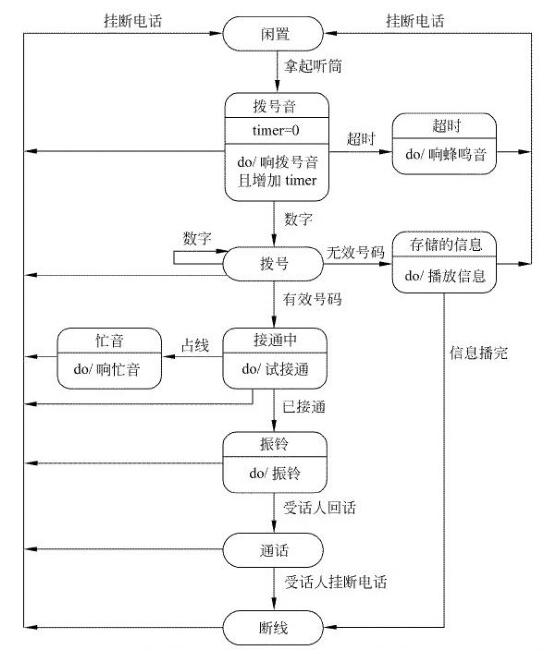
\includegraphics[width=0.6\textwidth]{状态转换图.jpg}
\end{figure}

\textbf{层次方框图}:用树形结构的一系列多层次的矩形框描述复杂数据的层次结构。

\begin{figure}[htbp]
    \centering
    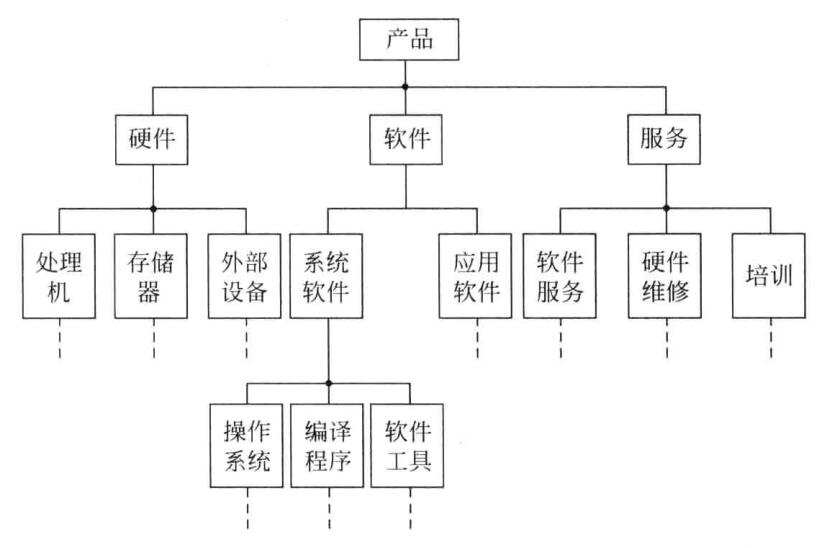
\includegraphics[width=0.6\textwidth]{层次方框图.jpg}
\end{figure}

\textbf{Warnier图}:与层次方框图类似,但提供了更丰富的描绘手段,可更清楚地描述信息的逻辑组织。

\begin{figure}[htbp]
    \centering
    \includegraphics[width=0.6\textwidth]{Warnier图.jpg}
\end{figure}

\subsection{验证软件需求}

\textbf{验证需求的一致性}:所有需求必须是一致的,任何一条需求不能和其他需求互相矛盾。

\textbf{验证需求的完整性}:需求必须是完整的,需求规格说明书中应包括用户需求的每一个功能或性能。

\textbf{验证需求的有效性}:必须证明需求是正确有效的,确实能够解决用户面对的问题。

\textbf{验证需求的现实性}:需求在现有硬件和软件技术水平上应该是能够实现的。

\section{总体设计}

复习内容:

\begin{enumerate}
    \item 掌握总体设计的设计原理
    \item 掌握软件结构设计的启发式规则
    \item 了解顺序图的作用及组成
\end{enumerate}

\subsection{总体设计过程}

总体设计的基本目的就是回答“概括地说,系统应该如何实现”这个问题,因此,总体设计又称为概要设计或初步设计。

总体设计的设计原理:\textbf{模块化、抽象、逐步求精、信息隐藏、模块独立}。

\textbf{模块化}:模块化的依据是使问题复杂度降低,易实现易理解。模块数目增加时每个模块的规模将减小,开发单个模块的工作量也将减少。但同时增加了设计模块接口的工作量。

\textbf{抽象}:将现实世界中具有共性的一类事物的相似的、本质的方面集中概括起来,而暂时忽略它们之间的细节差异。

\textbf{逐步求精}:为了能集中精力解决主要问题而尽量推迟对问题细节的考虑。逐步求精最初是自顶向下的设计策略,程序的体系结构通过逐步精化处理过程的层次设计出来。

\textbf{信息隐藏}:模块内部的信息对于不需要这些信息的模块来说是不能访问的。提高模块的独立性,模块之间的信息传递只能通过\textbf{合法的调用接口}来实现。

\textbf{模块独立}:模块独立的概念是模块化、抽象、信息隐蔽概念的直接结果。模块独立程度的度量标准:\textbf{耦合}:衡量\textbf{不同模块之间}相互依赖程度的度量指标;\textbf{内聚}:衡量\textbf{一个模块内部各元素}相互依赖程度的度量指标。

\textbf{耦合}

\begin{enumerate}
    \item \textbf{数据耦合}:如果两个模块彼此间通过参数交换信息,交换的信息只有数据。
    \item \textbf{控制耦合}:模块之间交换的信息中包含有控制信息。
    \item \textbf{特征耦合}:把整个数据结构作为参数传递而被调用的模块只需要使用其中一部分数据元素。
    \item \textbf{公共耦合}:两个或多个模块通过引用公共数据相互联系。
    \item \textbf{内容耦合}:一个模块访问另一模块的内部数据;一个模块不通过正常入口而转到另一模块内部;两个模块有一部分程序代码重叠;一个模块具有多个入口。
\end{enumerate}

数据耦合是低耦合,内容耦合是所有耦合关系中程度最高的。

\textbf{内聚}

\begin{enumerate}
    \item \textbf{偶然内聚}:一个模块完成一组任务,这些任务彼此间即使有关系,关系也是很松散的。
    \item \textbf{逻辑内聚}:一个模块完成的任务在逻辑上属相同或相似的一类。
    \item \textbf{时间内聚}:一个模块包含的任务必须在同一段时间内执行。
    \item \textbf{过程内聚}:一个模块内的处理元素是相关的,而且必须以特定次序执行。
    \item \textbf{通信内聚}:模块中所有元素都使用同一个输入数据和(或)产生同一个输出数据。
    \item \textbf{顺序内聚}:一个模块内的处理元素和同一个功能密切相关,而且这些处理必须顺序执行,通常前一部分的输出作为后一部分的输入。
    \item \textbf{功能内聚}:模块内所有处理元素属于一个整体,完成一个单一的功能。
\end{enumerate}

功能内聚是最高程度的内聚。

\subsection{启发式规则}

\textbf{改进软件结构提高模块独立性}:通过模块分解或合并,\textbf{降低耦合提高内聚}。

\textbf{模块规模应该适中}:一个模块的规模不应过大,通常不超过60行语句。

\textbf{深度、宽度、扇出和扇入都应适当}:顶层高扇出,中层低扇出,底层高扇入。

深度:软件结构中控制的层数,粗略地标示一个系统
的大小和复杂程度。

宽度:软件结构内同一个层次上模块总数的最大值,
一般来说,宽度越大的系统越复杂。

扇入:一个模块被多少个上级模块直接调用的数目。

扇出:一个模块直接控制(调用)的下级模块数目。

\textbf{模块的作用域应该在控制域范围之内}

作用域:受该模块内一个判定影响的所有模块范围。

控制域:模块本身及所有直接或间接从属于它的模块。

\textbf{力争降低模块接口的复杂程度}:模块接口设计原则是易理解,传递信息简单且与模块功能一致。

\textbf{设计单入口单出口的模块}:不要使模块间出现内容耦合。当从顶部进入模块并且从底部退出来时,软件是比较容易理解的,因此也是比较容易维护的。

\textbf{模块功能应该可以预测}:相同的输入应产生相同的输出。

\subsection{顺序图(时序图,序列图)}

顺序图是强调消息时间顺序的\textbf{交互图},描述了对象之间传送消息的时间顺序。顺序图阐明用例中的行为顺序,即说明对象如何通过交互来执行全部或部分用例的行为。

\textbf{对象}:类的实例,系统的参与者或者任何有效的系统对象。使用\textbf{显示对象名和类名的矩形框}来标记。

\textbf{生命线}:每个对象有自己的生命线,表示在该用例中一个对象在一段时间内的存在。即在生命线所代表的时间内,对象是可以被访问的。生命线位于每个对象的底部中心位置,使用\textbf{垂直的虚线}表示。交互过程中被销毁的对象,其生命线在接收到销毁对象消息时或在自身最后的返回消息之后结束,同时用一个“X”标记表明生命线的结束。

\textbf{激活}:表示对象执行一个动作所经历的时间段,也可表示对象在这段时间内不空闲,正在完成某个任务,或正被占用。激活在UML中用一个\textbf{细长的矩形}表示,显示在生命线上。矩形的顶部表示对象所执行动作的开始,底部表示动作的结束。对象在激活条的顶部被激活,在完成自己的工作后被去激活。去激活指对象处于空闲状态、在等待消息。

\textbf{消息}:面向对象方法中,消息是对象间交互信息的主要方式。消息是用来说明顺序图中不同活动对象之间的通信。消息表示为从一个对象的生命线指向另一个对象的生命线的\textbf{带箭头的实线},箭头上还可表明要发送的消息名及序号。顺序图中消息编号可显示,也可不显示。协作图中必须显示。\textbf{反身消息}是一个对象将一个消息发送给它自己。\textbf{返回消息}表示控制流从过程调用的返回,用\textbf{带箭头的虚线}表示。

顺序图的主要用途之一是把用例表达的要求转化为更进一步的精细表达。

\begin{figure}[htbp]
    \centering
    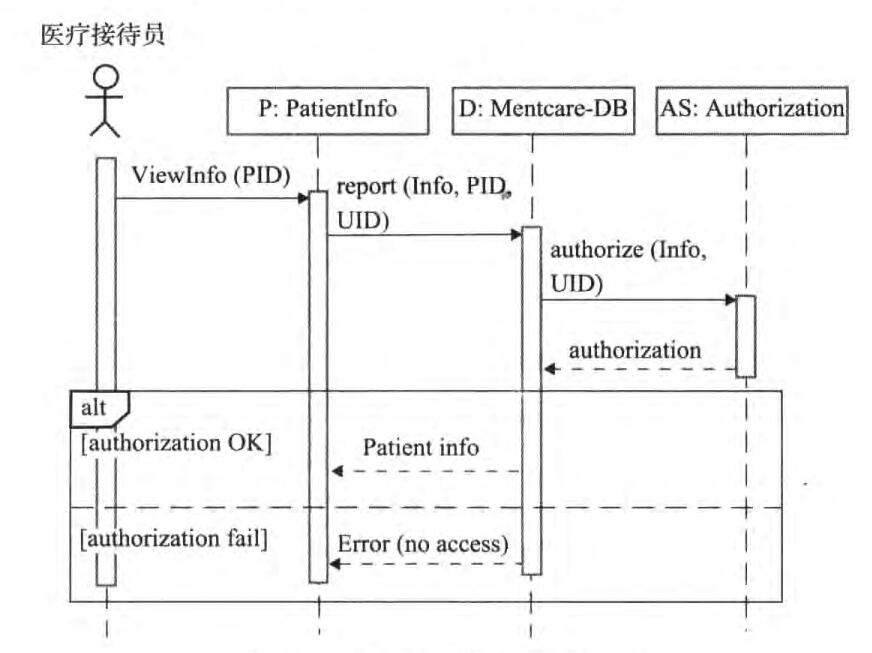
\includegraphics[width=0.8\textwidth]{顺序图.jpg}
\end{figure}

\section{详细设计}

复习内容:

\begin{enumerate}
    \item 了解结构程序设计的要求
    \item 掌握详细设计工具(程序流程图、盒图、PAD图)
\end{enumerate}

\subsection{结构程序设计的要求}

结构程序的经典定义:一个程序的代码块仅仅通过顺序、选择和循环这三种基本控制结构连接,并且每个代码块只有一个入口和一个出口。

结构程序设计更全面的定义:结构程序设计是尽可能少用 \lstinline{go to} 语句的程序设计方法。最好仅在检测出错误时才使用 \lstinline{go to} 语句,而且应该总是使用前向 \lstinline{go to} 语句。

理论上只用上述3种基本控制结构就可以实现任何单入口单出口的程序,但为了实际使用方便,还允许使用 \lstinline{do-until} 和 \lstinline{do-case} 两种控制结构。

经典的结构程序设计:只允许使用顺序、 \lstinline{if_then_else} 型分支和 \lstinline{do_while} 型循环这三种基本控制结构。

扩展的结构程序设计:除上述三种基本控制结构外,还允许使用 \lstinline{do-until} 型循环结构和 \lstinline{do-case} 型多分支结构。

修正的结构程序设计:再允许使用 \lstinline{break(leave)} 结构。

\subsection{详细设计工具}

详细设计工具分为图形、表格和语言三类。主要工具有:程序流程图、盒图(N-S图)、PAD图、判定表、判定树、过程设计语言(PDL)。

\textbf{程序流程图}

\begin{figure}[htbp]
    \centering
    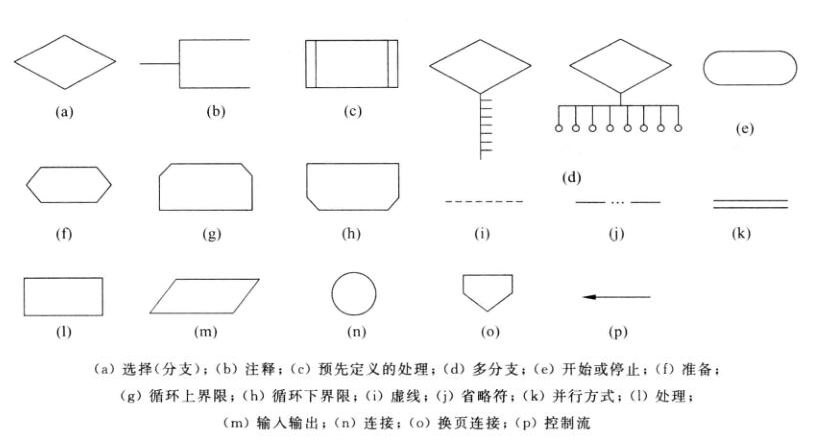
\includegraphics[width=0.75\textwidth]{程序流程图图例.jpg}
\end{figure}

\textbf{盒图(N-S图)}

\begin{figure}[htbp]
    \centering
    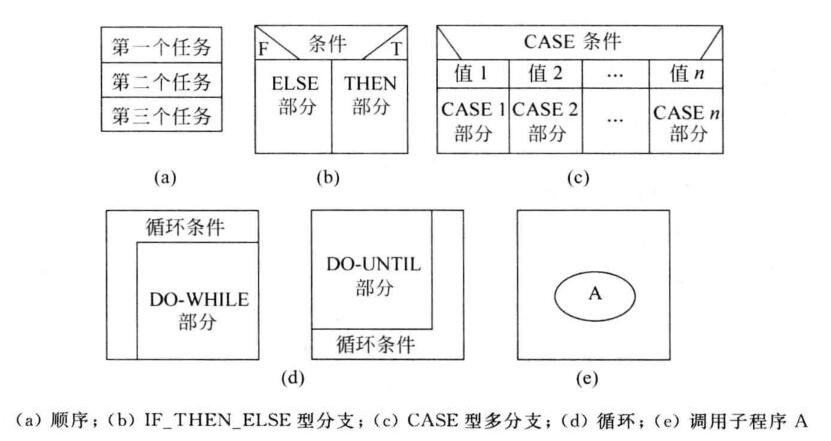
\includegraphics[width=0.8\textwidth]{盒图图例.jpg}
\end{figure}

\begin{figure}[htbp]
    \centering
    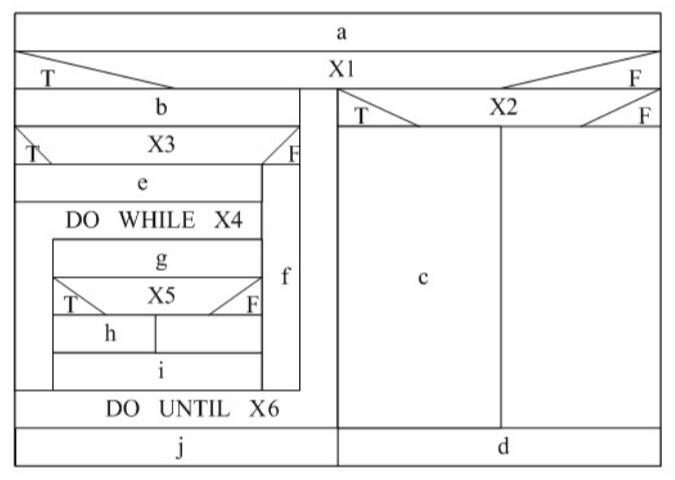
\includegraphics[width=0.5\textwidth]{盒图.jpg}
\end{figure}

\textbf{PAD图}

\begin{figure}[htbp]
    \centering
    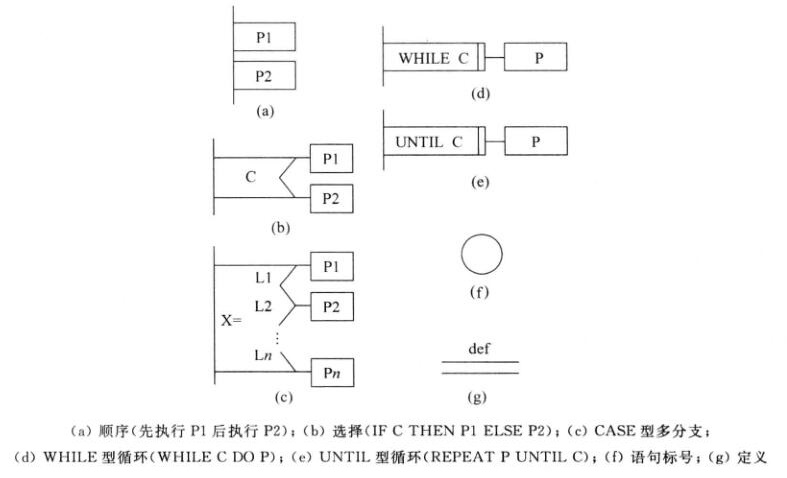
\includegraphics[width=0.75\textwidth]{PAD图图例.jpg}
\end{figure}

\begin{figure}[htbp]
    \centering
    \includegraphics[width=0.6\textwidth]{PAD图.jpg}
\end{figure}

\section{实现}

复习内容:

\begin{enumerate}
    \item 了解编码风格,测试的目的
    \item 了解白盒测试的概念,掌握不同覆盖标准测试用例的选择(语句、条件、路径)
    \item 了解黑盒测试的概念,了解三种黑盒测试方法
    \item 了解单元测试、集成测试、确认测试的目标和方法
\end{enumerate}

\subsection{编码风格与测试的目的}

代码应逻辑简明清晰、易读易懂。表现在以下方面:程序内部的文档(标识符、注解视觉组织),数据说明,语句构造,输入输出,效率。

测试是为了\textbf{发现程序中的错误}而执行程序的过程。成功的测试是发现了至今为止尚未发现的错误的测试。

测试方法:\textbf{黑盒测试}(又称\textbf{功能测试})把程序看作一个黑盒子,完全不考虑程序的内部结构和处理过程;\textbf{白盒测试}(又称\textbf{结构测试})是把程序看成装在一个透明的白盒子里,测试者完全知道程序的结构和处理算法。

\subsection{白盒测试}

\textbf{测试用例}:\textbf{测试数据和预期输出结果}。设计测试方案的基本目标是,确定一组最可能发现某个错误或某类错误的测试数据。

逻辑覆盖:\textbf{语句覆盖、判定覆盖、条件覆盖、判定/条件覆盖、条件组合覆盖}、点覆盖、边覆盖、路径覆盖。

\textbf{语句覆盖}:每个语句至少执行一次。

\textbf{判定覆盖}:又叫分支覆盖,不仅每个语句必须至少执行一次,而且每
个判定的每个分支都至少执行一次。

\textbf{条件覆盖}:不仅每个语句至少执行一次,而且使判定表达式中的每个条件都取到各种可能的结果。条件覆盖通常比判定覆盖强,但满足条件覆盖的测试数据不一定满足判定覆盖。

\textbf{判定/条件覆盖}:能同时满足判定覆盖和条件覆盖的逻辑覆盖。

\textbf{条件组合覆盖}:每个判定表达式中条件的各种可能组合都至少出现一次。条件组合覆盖是前述几种覆盖标准中最强的。

点覆盖:程序执行路径至少经过流图的每个结点一次,点覆盖标准和语句覆盖标准是相同的。

边覆盖:程序执行路径至少经过流图中每条边一次。通常边覆盖和判定覆盖是一致的。

路径覆盖:程序的每条可能路径都至少执行一次。路径覆盖相对来说是比较强的逻辑覆盖标准。但路径覆盖并没有检验表达式中条件的各种组合情况,而只考虑每个判定表达式的取值。

\subsection{黑盒测试}

\textbf{黑盒测试}着重测试\textbf{软件功能}。并不能取代白盒测试,与白盒测试互补,主要用于测试过程的\textbf{后期}。

\textbf{等价划分}

等价类划分:根据数据测试的等效性原理进行划分。

数据测试的等效性:分类的数据取其子集中一个数据做测试与子集中其他数据测试的效果是等效的。

\textbf{等价类}:某个输入域的子集合。在该子集合中,各个输入数据对于揭露程序中的错误都是等效的。

\textbf{有效等价类}:对于程序的规格说明来说,是合理的,有意义的输入数据构成的集合。

\textbf{无效等价类}:对程序的规格说明来说,是不合理的,无意义的输入数据构成的集合。

等价类划分方法:把程序的输入数据集合按输入条件划分为若干等价类,每个等价类相对于输入条件表示为一组有效或无效的输入,然后为每一等价类设计一个测试用例。确定输入等价类时还需分析输出数据的等价类,以便根据输出数据的等价类导出对应的输入等价类。

\begin{enumerate}
    \item 如果规定了输入值的范围,可划分出一个有效的等价类(输入值在此范围内),两个无效的等价类(输入值小于最小值或大于最大值)。
    \item 如果规定了输入数据的个数,则类似地也可以划分出一个有效的等价类和两个无效的等价类。
    \item 如果规定了输入数据的一组值,而且程序对不同输入值做不同处理,则每个允许的输入值是一个有效的等价类,此外还有一个无效的等价类(任一个不允许的输入值)。
    \item 如果规定了输入数据必须遵循的规则,则可划分出一个有效等价类(符合规则)和若干无效等价类(不同角度违反规则)。
    \item 如果输入条件是一个布尔量,则可以确定一个有效等价类和一个无效等价类。
    \item 如果规定了输入数据为整型,则可划分出正整数、零和负整数3个有效类。
    \item 如果程序的处理对象是表格,则应该使用空表,以及含一项或多项的表。
\end{enumerate}

划分出等价类以后,根据等价类设计测试方案时主要使用下面两个步骤:设计一个新的测试方案以\textbf{尽可能多地覆盖尚未被覆盖的有效等价类},重复这一步骤直到所有有效等价类都被覆盖为止。设计一个新的测试方案,使它\textbf{只覆盖一个尚未被覆盖的无效等价类},重复这一步骤直到所有无效等价类都被覆盖为止。

\textbf{边界值分析}

处理边界情况时程序最容易发生错误。使用边界值分析方法设计测试方案首先应该确定边界情况,通常输入等价类和输出等价类的边界。选取的测试数据应该刚好等于、刚刚小于和刚刚大于边界值。

\textbf{错误推测}

错误推测法在很大程度上靠直觉和经验进行。列举出程序中可能有的错误和容易发生错误的特殊情况,并且根据它们选择测试方案。在一段程序中已经发现的错误数目往往和尚未发现的错误数成正比。因此,在进一步测试时要着重测试那些已发现了较多错误的程序段。

\subsection{单元测试}

单元测试\textbf{集中检测软件设计的最小单元——模块}。单元测试主要使用白盒测试技术,辅以黑盒测试,而且对多个模块的测试可以并行地进行。可用人工测试和计算机测试两种不同类型的测试方法。

测试重点:模块接口、局部数据结构、重要的执行通路、出错处理通路、边界条件。

代码审查:由审查小组正式对源程序进行人工测试。审查小组的任务是发现错误而不是改正错误。

计算机测试:模块不是一个独立的程序,因此必须为每个单元测试开发驱动程序和(或)存根程序。驱动程序是一个“主程序”,它接收测试数据,启动被测模块,输出测试结果。存根程序代替被测试的模块所调用的模块,接收被测试模块的调用和输出数据。

\subsection{集成测试}

集成测试是\textbf{测试和组装软件}的系统化技术。

由模块组装成程序时有两种方法:\textbf{非渐增式测试方法、渐增式测试方法}。

\textbf{非渐增式测试方法}:先分别测试每个模块,再把所有模块按设计要求放在一起结合成所要的程序。

\textbf{渐增式测试方法}:把下一个要测试的模块同已经测试好的那些模块结合起来进行测试,测试完以后再把下一个应该测试的模块结合进来测试。这种方法实际上同时完成单元测试和集成测试。

\textbf{非渐增式测试}把所有模块放在一起作为一个整体来测试。测试时会遇到许多错误,\textbf{改正错误非常困难},因为在庞大的程序中想要诊断定位一个错误非常困难。\textbf{渐增式测试}把程序划分成小段来构造和测试,在这个过程中\textbf{比较容易定位和改正错误};对接口可以进行更彻底的测试。因此,目前集成测试时普遍采用渐增式测试方法。

当使用\textbf{渐增方式}把模块结合到程序中去时,有\textbf{自顶向下和自底向上}两种集成策略。

\textbf{自顶向下集成}:从主控制模块开始沿程序的控制层次向下移动,逐渐把各模块结合起来。把模块组装到程序结构中时可使用深度优先和宽度优先两种策略。

\textbf{自底向上集成}:从软件结构最低层模块开始组装和测试,当测试到较高层模块时,所需的下层模块均已具备,故不再需要桩模块。

\textbf{自顶向下测试方法}的主要优点是\textbf{不需要测试驱动程序},能够在测试阶段的早期实现并验证系统的主要功能,而且能在早期发现上层模块的接口错误。主要缺点是\textbf{需要存根程序},可能遇到与此相联系的测试困难,低层关键模块中的错误发现较晚,而且用这种方法在早期不能充分展开人力。自底向上测试方法的优缺点与自顶向下测试方法的优缺点相反。

\textbf{回归测试}:集成测试过程中,每当一个新模块结合进来时,程序就发生了变化。在集成测试的范畴中,回归测试指重新执行已经做过的测试的某个子集,以保证上述这些变化没有带来非预期的副作用。

\subsection{确认测试}

\textbf{确认测试}也称\textbf{验收测试},目标是\textbf{验证软件的有效性}。

\textbf{软件有效性}的一个简单定义是:如果软件的功能和性能如同用户所合理期待的那样,软件就是有效的。\textbf{软件需求规格说明书}是软件有效性的标准,也是进行确认测试的基础。

大多数软件开发商都使用\textbf{Alpha测试和Beta测试}的过程。

\textbf{Alpha测试}:由用户在开发者的场所进行,且在开发者“指导”下进行。开发者负责记录发现的错误和使用中遇到的问题,是在受控的环境中进行的。

\textbf{Beta测试}:由软件的最终用户们在一个或多个客户场所进行,是软件在开发者不能控制的环境中的“真实”应用。

\end{document}
